\documentclass[12pt, oneside, a4paper]{article}
% for math symbols
\usepackage{amsmath}
\usepackage{amssymb}
% for inserting images
\usepackage{graphicx}
% for algorithm pseudocode
\usepackage[noend]{algpseudocode}
\usepackage[nothing]{algorithm}
\algrenewcommand{\algorithmicrequire}{\textbf{Input:}}
\algrenewcommand{\algorithmicensure}{\textbf{Output:}}
\algnewcommand\And{\textbf{and} }
% for tables
\usepackage{tabularx}
% for implementation of the array and tabular environments
\usepackage{array}
% Control float placement. Defines a \FloatBarrier command
\usepackage{placeins}
% for derivative commands
\usepackage{physics}
% for multi level lists
\usepackage{outlines} 
% for links in text
\usepackage[colorlinks=true,linkcolor=blue,urlcolor=black,bookmarksopen=true]{hyperref} 
% for contents after pdf is formed
\usepackage{bookmark}
\usepackage{xcolor}
% for code in text
\usepackage{listings}
\usepackage{pythonhighlight}
 

\newcommand{\vect}[1]{\ensuremath{\mathbf{#1}}}
\newcommand{\vt}[1]{\ensuremath{\mathbf{#1}}}
\newcommand{\uline}[1]{\underline{#1}}
\newcommand{\tb}[1]{\textbf{#1}}
\newcommand{\ilcode}{\texttt}
\newcommand{\p}{\partial}
\newcommand{\vphi}{\varphi}

\DeclareUnicodeCharacter{2212}{\textendash}

\graphicspath{ {./images/} }

\title{CSDS 341: Final Project Report\\ Questionnaire Website}
\author{Oleksii Fedorenko, David Frost, Matthew Garcia, Preeti Naik}

\begin{document}
    \maketitle
    %%%%%%%%%%%%%%%%%%%%%%%%%%%%%%%%%%%%%%%%%%%%%%%%%%%%%%%%%%%%%%%%%%%%%%%%%%
    %%%%%%%%%%%%%%%%%%%%%%%%%%%%%%%%%%%%%%%%%%%%%%%%%%%%%%%%%%%%%%%%%%%%%%%%%%
    %%%%%%%%%%%%%%%%%%%%%%%%%%%%%%%%%%%%%%%%%%%%%%%%%%%%%%%%%%%%%%%%%%%%%%%%%%
    \section{Background}
    Questionnaires and surveys are very important for understanding and shaping the world. Surveys are one of the main tools for collection and analysis of data for making decisions. For example, United States uses the Census and the American Community Survey to understand how country demographics is shifting and to make decisions about the allocation of resources. Researchers use questionnaires for scientific studies to understand both the social and natural worlds. Psychologists in particular make great use of Likert scales in questionnaires to help build our collective knowledge. 
    \newline\newline\indent Therefore, streamlining the process of collecting and analysing surveys using technology is very beneficial for decision-making. Our application would allow users to create their own questionnaires, distribute and analyse them easily. Additionally, application would allow for streamlining the decision-making process based on the analysis of data to an advanced degree.
    \newline\newline\indent This will be accomplished through the design of the database allowing for multiple functionalities based on the user. With different roles and permissions a user will be able to participate in questionnaires or be the creator of a questionnaire. Then, questionnaires will have a certain amount of questions and these questions will have possible answers created by the maker of the questionnaire. Responses will be recorded and using the relationships in the database queries can be written to analyze the gathered data. This survey tool streamlines the process of creating and answering surveys and allows for data analysis to make decisions or understand the participants choices.
    %%%%%%%%%%%%%%%%%%%%%%%%%%%%%%%%%%%%%%%%%%%%%%%%%%%%%%%%%%%%%%%%%%%%%%%%%%
    %%%%%%%%%%%%%%%%%%%%%%%%%%%%%%%%%%%%%%%%%%%%%%%%%%%%%%%%%%%%%%%%%%%%%%%%%%
    %%%%%%%%%%%%%%%%%%%%%%%%%%%%%%%%%%%%%%%%%%%%%%%%%%%%%%%%%%%%%%%%%%%%%%%%%%
    \section{Data Description}
    \emph{Users} contains information about all of the users, questionnaire creators and reponders, that interact with the website. This data will be obtained through a registration form on the website for creating accounts that asks users for their names, emails, region, and subscription type. At minimum, every user must have at least an email since it serves as a unique identifier that allows them to log in, so the email attribute of \emph{Users} is UNIQUE and NOT NULL.
    \\
    \\
    \emph{Permissions} contains information about all of the permission levels of users for each questionnaire. This data is generated when a questionnaire is made and then the creator of the questionnaire specifies the permissions for the questionnaire for everyone else as they have control over whether other people can view, answer, or edit their questionnaire. \emph{Users} and \emph{Roles} do not have full participation in this ternary relationship.
    \\
    \\
    \emph{Roles} contains information about all of the roles available on the questionnaire website. Each user that is related to a particular questionnaire must have a particular role. However, not every user is related to a particular questionnaire. There are seven different roles we have implemented: \emph{root}, which has all permissions, \emph{creator}, which is for the creators of questionnaires who can edit the questionnaire and view responses but cannot answer their own questionnaire, \emph{moderator}, which can only edit the questionnaire but cannot answer it or view responses, \emph{participant}, which can only respond, \emph{analyst}, which can only view responses, and \emph{guest}, which has no permissions. These roles only need to be added once but there is a table for roles to reduce redundancy. Therefore, we do not expect more tuples to be added to this table unless added by the website's administrator.
    \\
    \\
    \emph{Subscription} is the table that holds all of the info about all of the subscriptions available on the website. Users are limited about how many surveys they are allowed to create depending on their subscription plan. subscription\_id is the primary key and each subscription level has a unique id. Each subscription also has a survey\_limit associated with it that is the number of surveys a user with that subscription is allowed to create. This data is generated only by the administrator of the website as tuples are only added, updated, or deleted whenever the admin changes the subscription offering.
    \\
    \\
    \emph{Questionnaires} is the table that contains all questionnaires for the website. questionnaire\_id is the primary key of Questionnaires. Each questionnaire is made by users and when a user creates a questionnaire they are automatically added in the permissions table as being a creator for that questionnaire\_id.  The attribute number\_of\_questions is to hold how many questions the questionnaire contains.
    \\
    \\
    \emph{Questions} contains all of the questions associated with their specific questionnaire. The questions are made by users when creating a questionnaire, and the primary key for Questions is question\_id. When a question is created it has a foreign key questionnaire\_id to associate it with the correct questionnaire that the question originates from. The attribute question\_text contains the text of the question.
    \\
    \\
    \emph{Possible\_Answers} contains all possible answers for a question. The primary key for a possible answer is option\_id. When a possible answer is created it has a foreign key question\_id to associate it with the proper question that the possible answer should be under. The attribute possible\_answer contains the text of the possible answer.
    \\
    \\
    \emph{Responses} contains all of the selected possible answers by each user for a questionnaire. The primary key for Responses is response\_id. The foreign key user\_id points to the correct user that selected the response. The foreign key option\_id shows which option the user had selected by linking it to the possible answer. The attribute date\_time lets us know what time the user had selected their response.
    \\
    \\
    \emph{Data Generation}
    We took an approach of generating data for tables with least dependencies at first. Those are: Roles and Subscription. Then, we generated data for Users, using random name generator plugin and using Subscription table. Then, we used random questions from the internet to generate Quesionnaires, which randomly chose questions from the list of random Questions. Then, using the generated Questions table, we used random string generator to generate Possible Answers. Using the tables for Questionnaires, Roles and Users, we generated creators, moderators and participants for each questionnaire. Based on the participant roles in the Permissions table, we randomly selected responses to the corresponding Questionnaires and Answers for each participant in a given Questionnaire. The responses were recorded in the Responses table. 

    Since our project depends on user-generated data, we had to artificially generate random data to demonstrate how our database works. We generated data using a Python script which created hundreds of users with random names, multiple choice possible answers to questions, and responses to questions and questionnaires.
    %%%%%%%%%%%%%%%%%%%%%%%%%%%%%%%%%%%%%%%%%%%%%%%%%%%%%%%%%%%%%%%%%%%%%%%%%%
    %%%%%%%%%%%%%%%%%%%%%%%%%%%%%%%%%%%%%%%%%%%%%%%%%%%%%%%%%%%%%%%%%%%%%%%%%%
    %%%%%%%%%%%%%%%%%%%%%%%%%%%%%%%%%%%%%%%%%%%%%%%%%%%%%%%%%%%%%%%%%%%%%%%%%%
    \section{ER\ Diagram}
    \FloatBarrier
    \begin{figure}[H] 
        \centerline{
        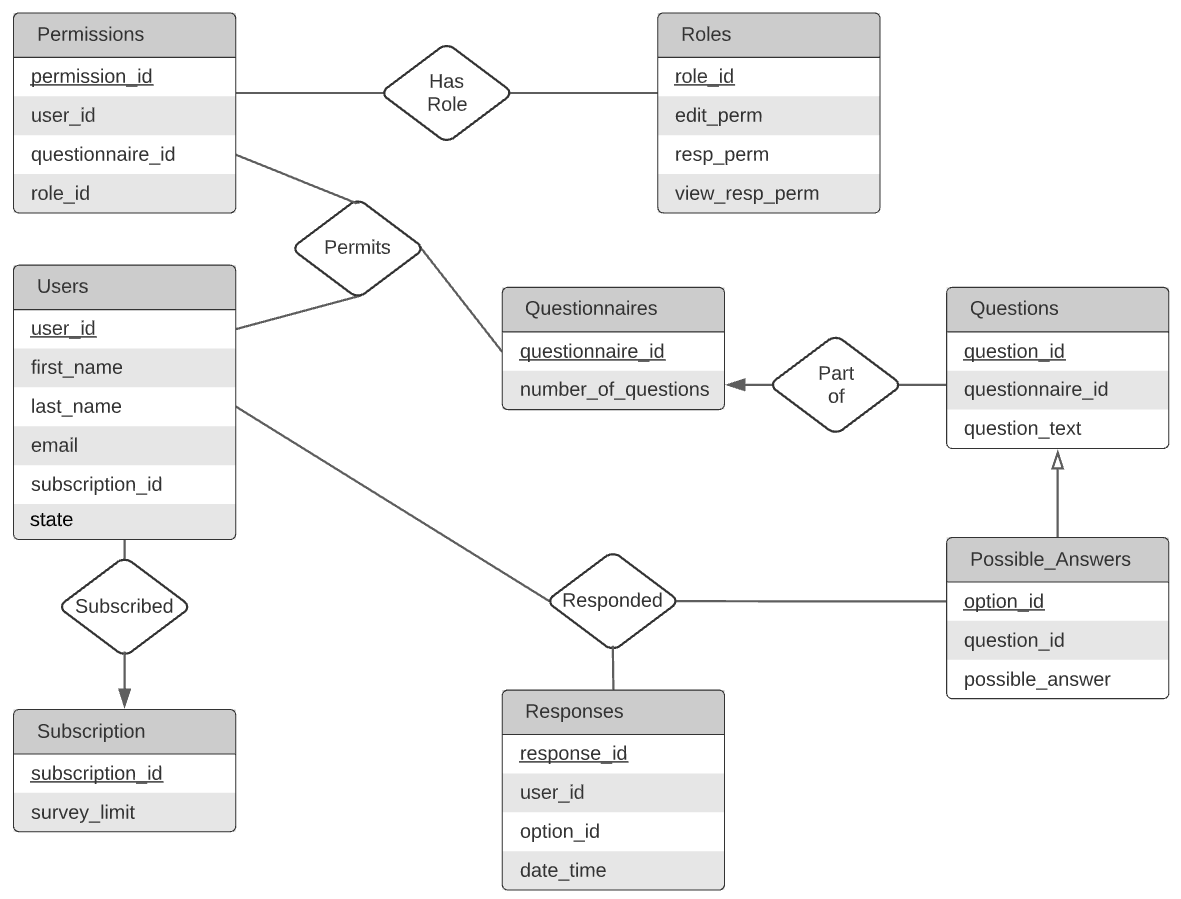
\includegraphics[width=\textwidth]{newERdiagram.PNG}
        }
    \end{figure}
    \newpage
    %%%%%%%%%%%%%%%%%%%%%%%%%%%%%%%%%%%%%%%%%%%%%%%%%%%%%%%%%%%%%%%%%%%%%%%%%%
    %%%%%%%%%%%%%%%%%%%%%%%%%%%%%%%%%%%%%%%%%%%%%%%%%%%%%%%%%%%%%%%%%%%%%%%%%%
    %%%%%%%%%%%%%%%%%%%%%%%%%%%%%%%%%%%%%%%%%%%%%%%%%%%%%%%%%%%%%%%%%%%%%%%%%%
    \section{Functional Dependencies and BCNF}
    \tb{Users} \\
    This entity represents users of the questionnaire website.
    All types of users, including people who create questionnaires
    or answer questionnaires, are in this table. first\_name, last\_name, email, subscription\_id are attributes of the User and there is no FD between them except that email determines everything else since it is a candidate key as no two users can have the same email address. \\
    R1 = (user\_id, first\_name, last\_name, email, subscription\_id) \\
    F1 = \{user\_id \(\rightarrow\) first\_name, last\_name, email, subscription\_id; email \(\rightarrow\) user\_id, first\_name, last\_name, subscription\_id\} \\
    Since, both user\_id and email are superkeys Users is in BCNF form. 
    \\

    \tb{Permissions} \\
    This entity describes the permission level of a user for each 
    questionnaire, this is part of a ternary relationship between users, questionnaire, and permission. user\_id, questionnaire\_id, role\_id are attributes of Permission and there is no FD in between them. \\
    R2 = (permission\_id, user\_id, questionnaire\_id, role\_id) \\
    F2 = \{permission\_id \(\rightarrow\) user\_id, questionnaire\_id, role\_id\} \\
    Since permission\_id is a superkey Permissions is in BCNF form. 
    \\
    
    \tb{Roles} \\
    This entity describes the roles that are allowed for each permission evel. For each role there are different permissions that are dependent on a true or false value (BIT) in SQL. For each tuple of user and survey the permission level determines what roles they have. edit\_perm, resp\_perm, view\_resp\_perm are all attributes of a role with no FD between them. \\
    R3 = (role\_id, edit\_perm, resp\_perm, view\_resp\_perm) \\
    F3 = \{role\_id \(\rightarrow\) edit\_perm, resp\_perm, view\_resp\_perm\} \\
    Since role\_id is a superkey Roles is in BCNF form. 
    \\

    \tb{Subscription} \\
    Describes the subscription level and how many surveys users are allowed to create at each subscription level. \\
    R4 = (subscription\_id, survey\_limit) \\
    F4 = \{subscription\_id \(\rightarrow\) survey\_limit\} \\
    Since subscription\_id is a superkey Subscription is in BCNF form. 
    \\

    \tb{Questionnaires} \\
    Defines a questionnaire with the unique id that will be bound to a user using the permissions table. \\
    R5 = (questionnaire\_id, number\_of\_questions) \\
    F5 = \{questionnaire\_id, number\_of\_questions\} \\ 
    Since questionnaire\_id is a superkey Questionnaires is in BCNF form. 
    \\

    \tb{Questions} \\
    Determines questions as they are related to each questionnaire. questionnaire\_id, question\_text are attributes of Question with no FD between them. \\
    R5 = (question\_id, questionnaire\_id, question\_text) \\
    F5 = \{question\_id \(\rightarrow\) questionnaire\_id, question\_text\} \\
    Since question\_id is a superkey Questions is in BCNF form. 
    \\

    \tb{Possible\_Answers} \\
    Defines possible answers to each question. e.g. for multiple choice questions, this will have entries for each possible answer, while for questions like rating questions, this place will have the range of rankings available. question\_id, possible\_answer are attributes of an response option with no FD between them. \\
    R6 = (option\_id, question\_id, possible\_answer) \\
    F6 = \{option\_id \(\rightarrow\) question\_id, possible\_answer\} \\
    Since option\_id is a superkey Possible\_Answers is in BCNF form. 
    \\

    \tb{Responses} \\
    Defines the user response to each of the questions and ties them to the unique response option identifier and user id. user\_id, option\_id, date\_time have no FD between them. \\
    R7 = (response\_id, user\_id, option\_id, date\_time) \\
    F7 = \{response\_id $\rightarrow$ user\_id, option\_id, date\_time\} \\
    Since response\_id is a superkey Responses is in BCNF form. 
    \\
    %%%%%%%%%%%%%%%%%%%%%%%%%%%%%%%%%%%%%%%%%%%%%%%%%%%%%%%%%%%%%%%%%%%%%%%%%%
    %%%%%%%%%%%%%%%%%%%%%%%%%%%%%%%%%%%%%%%%%%%%%%%%%%%%%%%%%%%%%%%%%%%%%%%%%%
    %%%%%%%%%%%%%%%%%%%%%%%%%%%%%%%%%%%%%%%%%%%%%%%%%%%%%%%%%%%%%%%%%%%%%%%%%%
    \section{Schemas}
    \begin{lstlisting}[language=SQL, columns=flexible, breaklines]
        CREATE TABLE Users
        (
            user_id INT AUTO_INCREMENT,
            first_name VARCHAR(40),
            last_name VARCHAR(40),
            email VARCHAR(100) NOT NULL UNIQUE,
            subscription_id INT,
            state VARCHAR(10),
            PRIMARY KEY(user_id),
            FOREIGN KEY(subscription_id) REFERENCES Subscription(subscription_id) ON DELETE CASCADE
        );
    \end{lstlisting}
    \begin{lstlisting}[language=SQL, columns=flexible, breaklines]
    CREATE TABLE Permissions
    (
        permission_id INT AUTO_INCREMENT,
        user_id INT,
        questionnaire_id INT,
        role_id varchar(30),
        PRIMARY KEY (permission_id),
        FOREIGN KEY(user_id) REFERENCES Users(user_id) ON DELETE CASCADE,
        FOREIGN KEY(questionnaire_id) REFERENCES Questionnaires(questionnaire_id) ON DELETE CASCADE,
        FOREIGN KEY(role_id) REFERENCES Roles(role_id) ON DELETE CASCADE
    );
    \end{lstlisting}
    \begin{lstlisting}[language=SQL, columns=flexible, breaklines]
    CREATE TABLE Roles
    (
        role_id varchar(30),
        edit_perm BIT,
        resp_perm BIT,
        view_resp_perm BIT,
        PRIMARY KEY(role_id)
    );
    \end{lstlisting}
    \begin{lstlisting}[language=SQL, columns=flexible, breaklines]
    CREATE TABLE Subscription
    (
        subscription_id INT AUTO_INCREMENT,
         survey_limit INT,
        PRIMARY KEY(subscription_id)
    );
    \end{lstlisting}
    \begin{lstlisting}[language=SQL, columns=flexible, breaklines]
    CREATE TABLE Questionnaires
    (
        questionnaire_id INT AUTO_INCREMENT,
        number_of_questions INT,
        PRIMARY KEY(questionnaire_id)
    );
    \end{lstlisting}
    \begin{lstlisting}[language=SQL, columns=flexible, breaklines]
    CREATE TABLE Questionnaires
    (
        questionnaire_id INT AUTO_INCREMENT,
        number_of_questions INT,
        PRIMARY KEY(questionnaire_id)
    );
    \end{lstlisting}
    \begin{lstlisting}[language=SQL, columns=flexible, breaklines]
    CREATE TABLE Questions
    (
        question_id BIGINT AUTO_INCREMENT,
        questionnaire_id INT,
        question_text VARCHAR(400),
        PRIMARY KEY(question_id),
        FOREIGN KEY(questionnaire_id) REFERENCES Questionnaires(questionnaire_id) ON DELETE CASCADE
    );
    \end{lstlisting}
    \begin{lstlisting}[language=SQL, columns=flexible, breaklines]
    CREATE TABLE Possible_Answers
    (
        option_id BIGINT AUTO_INCREMENT,
        question_id BIGINT,
        possible_answer VARCHAR(400),
        PRIMARY KEY(option_id),
        FOREIGN KEY(question_id) REFERENCES Questions(question_id) ON DELETE CASCADE
    );
    \end{lstlisting}
    \begin{lstlisting}[language=SQL, columns=flexible, breaklines]
    CREATE TABLE Responses
    (
        response_id INT AUTO_INCREMENT,
        user_id INT,
        option_id BIGINT,
        date_time DATETIME,
        PRIMARY KEY(response_id),
        FOREIGN KEY(user_id) REFERENCES Users(user_id) ON DELETE CASCADE,
        FOREIGN KEY(option_id) REFERENCES Possible_Answers(option_id) ON DELETE CASCADE
    );
    \end{lstlisting}
    %%%%%%%%%%%%%%%%%%%%%%%%%%%%%%%%%%%%%%%%%%%%%%%%%%%%%%%%%%%%%%%%%%%%%%%%%%
    %%%%%%%%%%%%%%%%%%%%%%%%%%%%%%%%%%%%%%%%%%%%%%%%%%%%%%%%%%%%%%%%%%%%%%%%%%
    %%%%%%%%%%%%%%%%%%%%%%%%%%%%%%%%%%%%%%%%%%%%%%%%%%%%%%%%%%%%%%%%%%%%%%%%%%
    \section{Example Queries}
    \subsection*{Query 1}
    \noindent Find the number of responses to a specific question. Replace the first predicate in WHERE to specify which question. Query in SQL:
    \begin{lstlisting}[language=SQL, columns=flexible, breaklines]
        SELECT count(r.response_id)
        FROM Questions as q, Possible_Answers as p, Responses as r
        WHERE q.question_id = "question_id" AND p.question_id = q.question_id AND r.option_id = p.option_id
    \end{lstlisting}
    \noindent Query in relational algebra:\\
    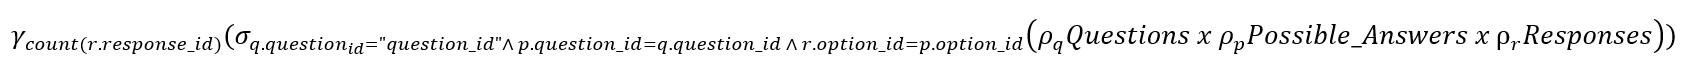
\includegraphics{responsecountqueryalgebra.PNG}
    \noindent Result of running this query with q.question\_id = 1:
    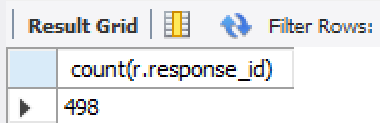
\includegraphics{responsecountquery.PNG}

    \subsection*{Query 2}
    \noindent Find all of the questions that were responded to by people from a specific state and show what multiple choice answer they picked. Change state as necessary, it is Illinois for example here:
    \begin{lstlisting}[language=SQL, columns=flexible, breaklines]
        SELECT q.question_text, p.possible_answer as answer, u.user_id, first_name, last_name, state
        FROM Users u, Responses r, Questions q, Possible_Answers p
        WHERE r.option_id = p.option_id AND p.question_id = q.question_id AND u.user_id = r.user_id AND state = "IL";
    \end{lstlisting}
    \noindent Query in relational algebra: \\
    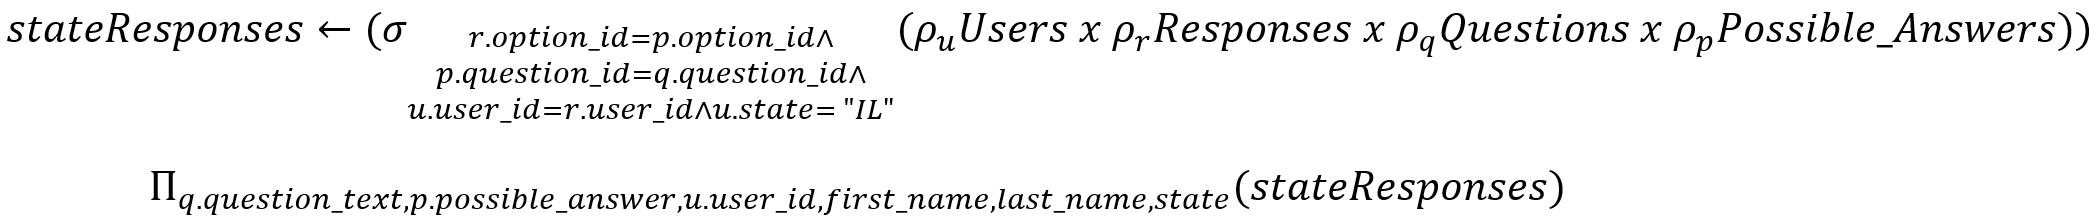
\includegraphics[scale=0.6]{questionstatequeryalgebra.PNG}
    \noindent Query in tuple relational calculus: \\
    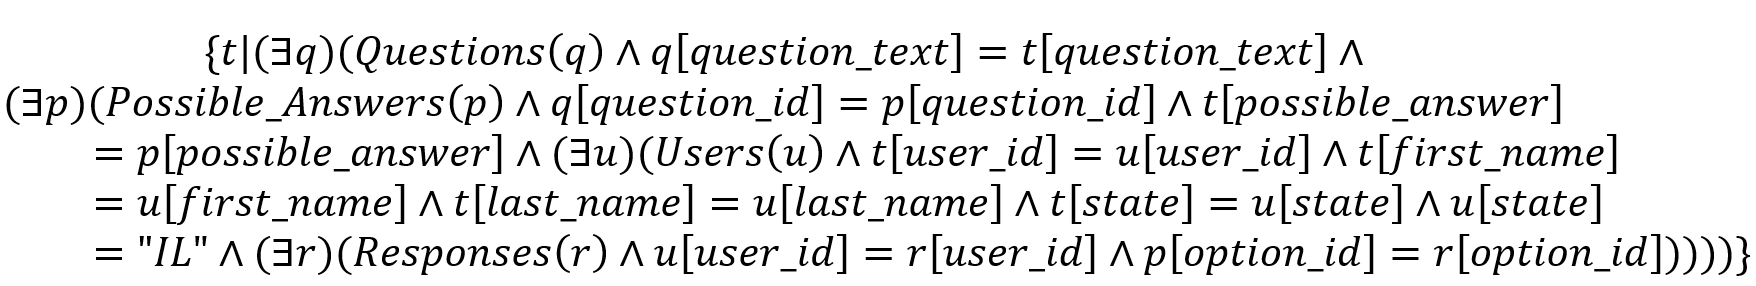
\includegraphics[scale=0.7]{questionstatequerycalculus3.PNG}
    Result of running this query with state = "IL":\\
    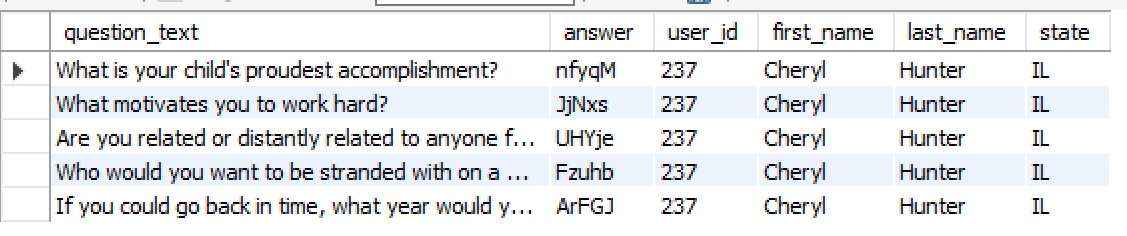
\includegraphics{questionstatequeryresult.PNG}

    \subsection*{Query 3}
    \noindent Retrieve user answers for a specific questionnaire.
    \begin{lstlisting}[language=SQL, columns=flexible, breaklines]
        SELECT r.option_id, r.date_time
        FROM Questionnaires as q, Questions as q2, Possible_Answers as p, Responses as r
        WHERE r.option_id = p.option_id 
            AND p.question_id = q2.question_id 
            AND q.questionnaire_id = q2.questionnaire_id
            AND q.questionnaire_id = "QuestionnaireID"
            AND r.user_id = "UserID";
    \end{lstlisting}
    \noindent Query in relational algebra: 
    \begin{align*}
        \Pi&_{r.option\_id,\ r.date\_time}(\sigma_{q.questionnaire\_id\ =\ "QuestionnaireID"\ \wedge\ r.user\_id\ =\ "UserID"}
        (\\
        &\rho_{q}Questionnaires\ \bowtie\ \rho_{q2}Questions\ \bowtie\ \rho_{p}Possible\_Answers\ \bowtie\ \rho_{r}Responses\\
        ))&
    \end{align*}
    
    \bigskip
    \noindent \noindent \noindent Query in tuple relational calculus: 
    \begin{align*}
        \{t\ |\ (&\exists r)\ (r\ \in\ Responses\ \wedge\ t[option\_id] = r[option\_id]\ \wedge\ t[date\_time] = r[date\_time]\\
        \newline\wedge\ (&\exists p)\ (p\ \in\ Possible\_Answers\ \wedge\ r[option\_id]=p[option\_id]\\
        \newline\wedge\ (&\exists q2)\ (q2\ \in\ Questions\ \wedge\ p[question\_id] = q2[question\_id]\\
        \newline\wedge\ (&\exists q)\ (q\ \in\ Questionnaires\ \wedge\ q2[questionnaire\_id] = q[questionnaire\_id]\ \wedge\ \\
        &r.user\_id\ =\ "UserID"\ \wedge\ q.questionnaire\_id\ =\ "QuestionnaireID"))))\}
    \end{align*}
    \noindent Result of running this query:\\
    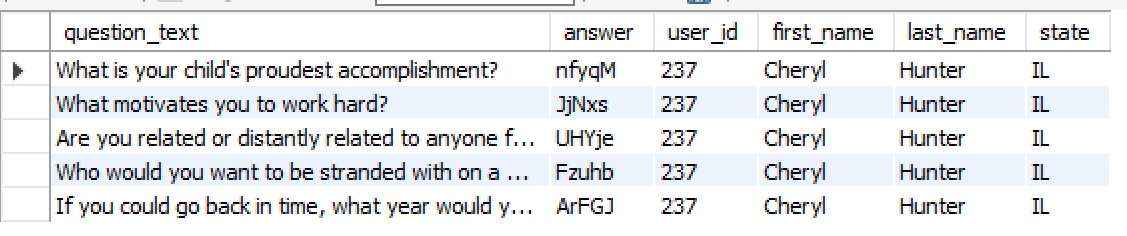
\includegraphics{questionstatequeryresult.PNG}
    %%%%%%%%%%%%%%%%%%%%%%%%%%%%%%%%%%%%%%%%%%%%%%%%%%%%%%%%%%%%%%%%%%%%%%%%%%
    %%%%%%%%%%%%%%%%%%%%%%%%%%%%%%%%%%%%%%%%%%%%%%%%%%%%%%%%%%%%%%%%%%%%%%%%%%
    %%%%%%%%%%%%%%%%%%%%%%%%%%%%%%%%%%%%%%%%%%%%%%%%%%%%%%%%%%%%%%%%%%%%%%%%%%

    \section{Implementation}
    We used MySQL as our database management system. We used Python to create a console app that allows for many interactions with the system from the command line, such as adding a new user, viewing the list of questionnaires on the website, answering a questionnaire, viewing the answers to a particular questionnaire, and creating a questionnaire. This Python app uses MySQL Connector to connect to MySQL, so it may be necessary to run \emph{python -m pip install mysql-connector-python}. We also started developing a Python Flask app using SQLAlchemy to connect to the MySQL database. To run this app, you need to go to the directory csds341\_server and then run \emph{pip install -r requirements.txt} to be able to run it, and then run \emph{flask run}, and then go to your web browser of choice and visit 127.0.01:5000 or localhost:5000 to see it.
    \section{Demo}
    We did a presentation in the last week of class. The slides are in the writeup folder in a file called "CSDS 341 Project Presentation".pdf. We also did a demo to our TA where we showed him our schemas which were significantly updated from our initial report with many additional constraints. We showed him that we successfully created our MySQL database for the project named "csds341\_questionnaire" and our progress on our Flask web app and our Python console app for interacting with the questionnaire system from the command line. We also showed him our sample queries and the successful results of running them.

    %%%%%%%%%%%%%%%%%%%%%%%%%%%%%%%%%%%%%%%%%%%%%%%%%%%%%%%%%%%%%%%%%%%%%%%%%%
    %%%%%%%%%%%%%%%%%%%%%%%%%%%%%%%%%%%%%%%%%%%%%%%%%%%%%%%%%%%%%%%%%%%%%%%%%%
    %%%%%%%%%%%%%%%%%%%%%%%%%%%%%%%%%%%%%%%%%%%%%%%%%%%%%%%%%%%%%%%%%%%%%%%%%%
    \section{WEB App}
    \FloatBarrier
    \begin{figure}[H] 
        \centerline{
        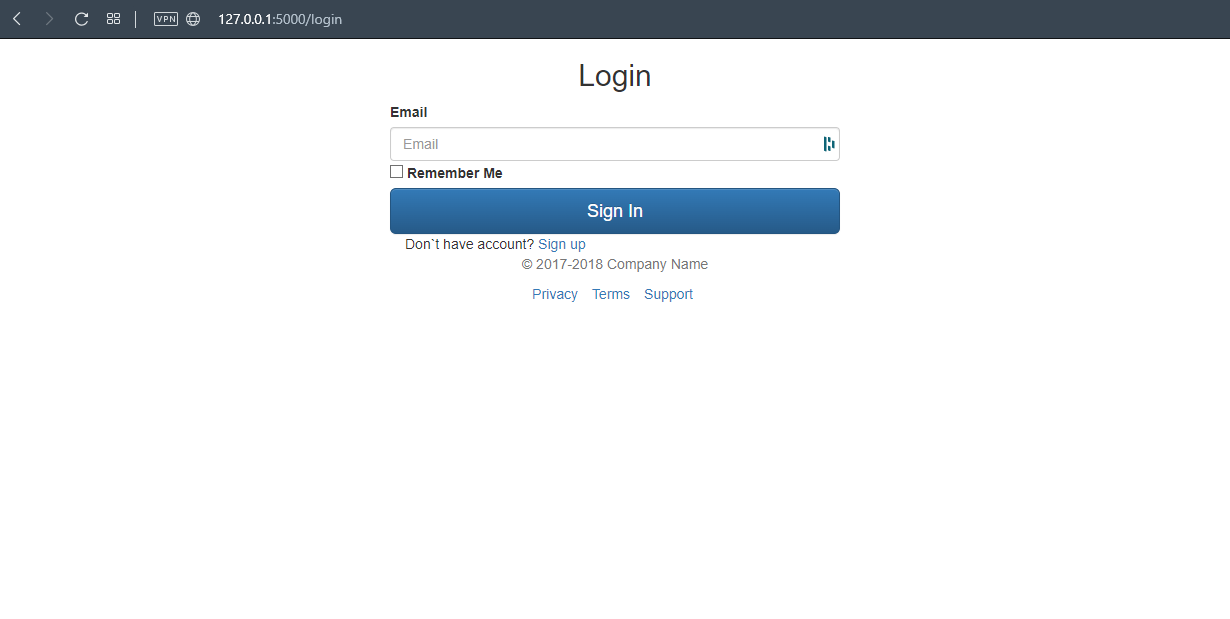
\includegraphics[width=\textwidth]{web_login.PNG}
        }
    \end{figure}
    \FloatBarrier
    \begin{figure}[H] 
        \centerline{
        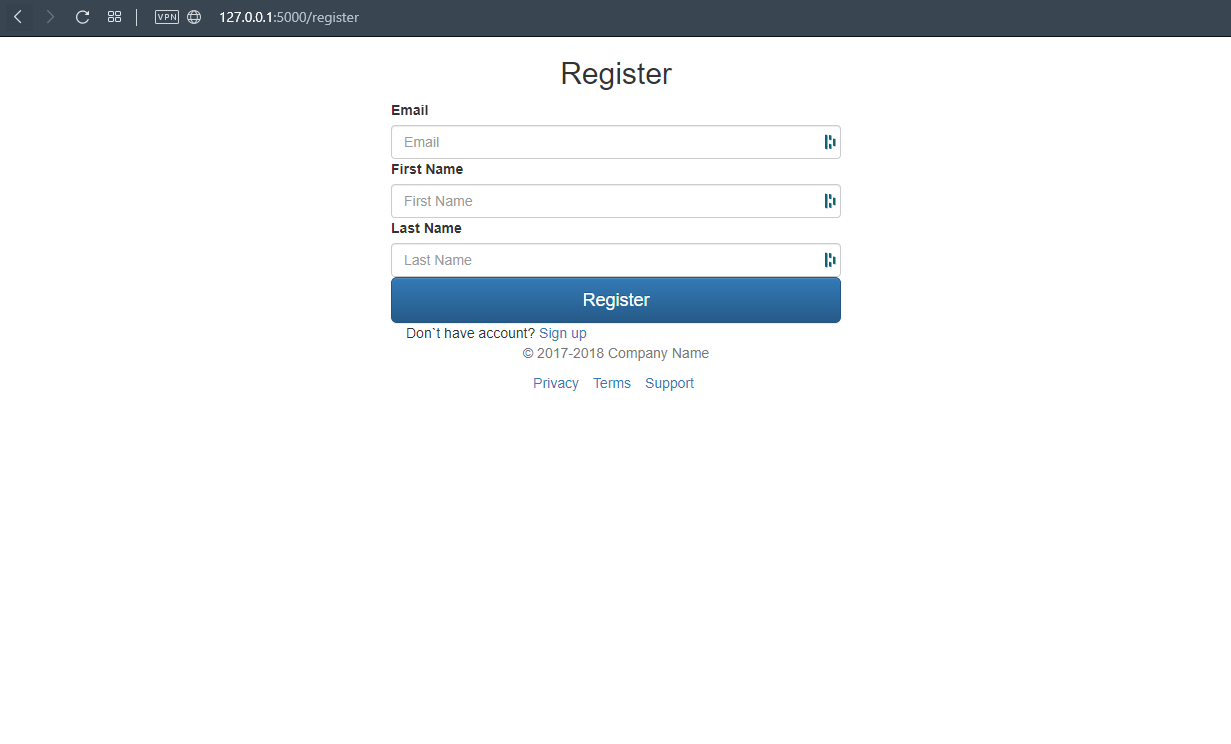
\includegraphics[width=\textwidth]{web_register.PNG}
        }
    \end{figure}
    \FloatBarrier
    \begin{figure}[H] 
        \centerline{
        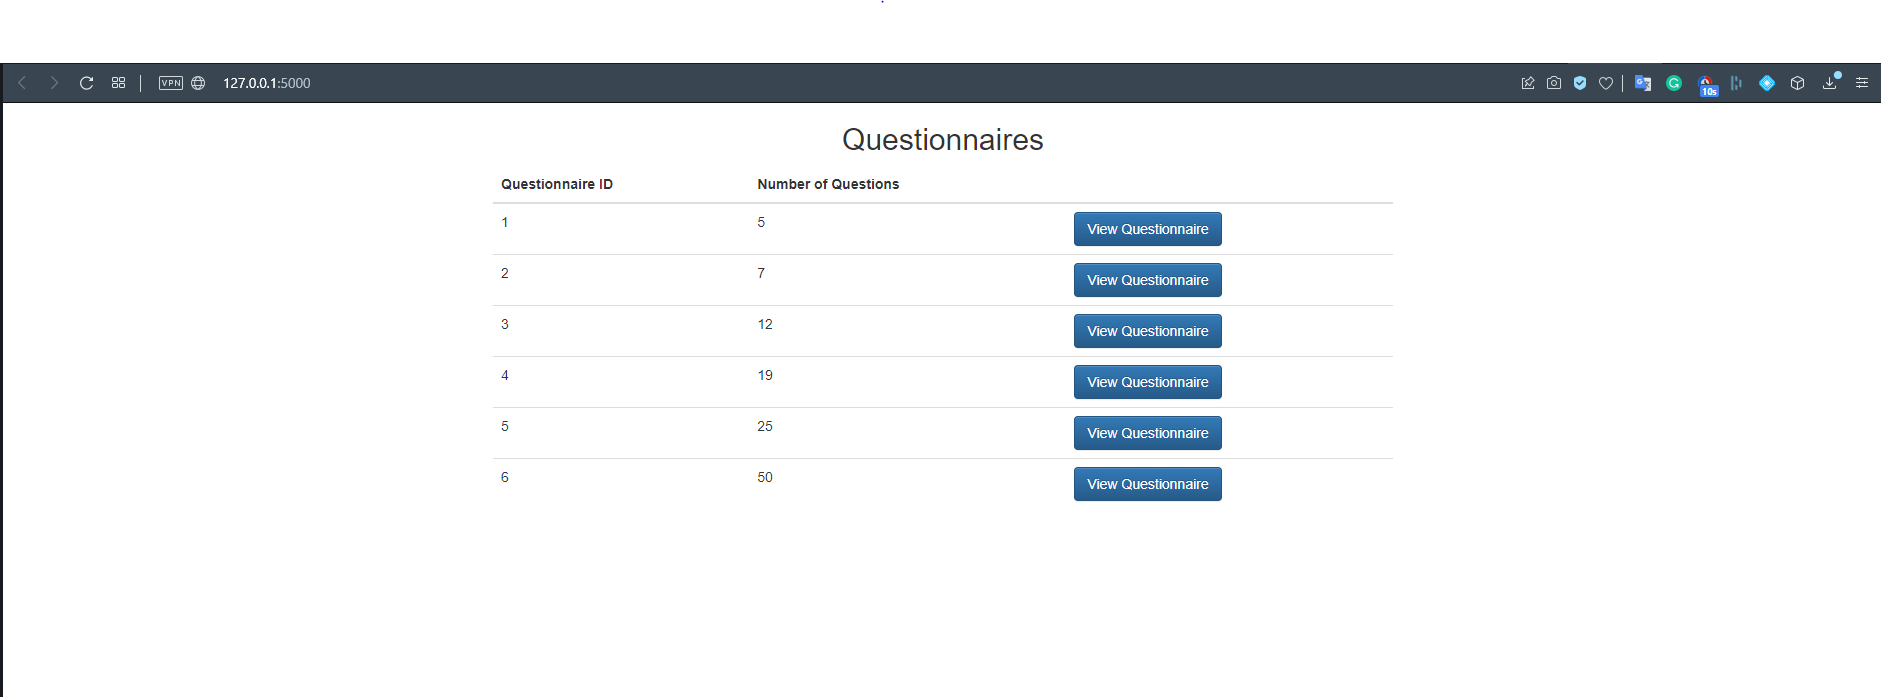
\includegraphics[width=\textwidth]{web_questionnaires.PNG}
        }
    \end{figure}
    \FloatBarrier
    \begin{figure}[H] 
        \centerline{
        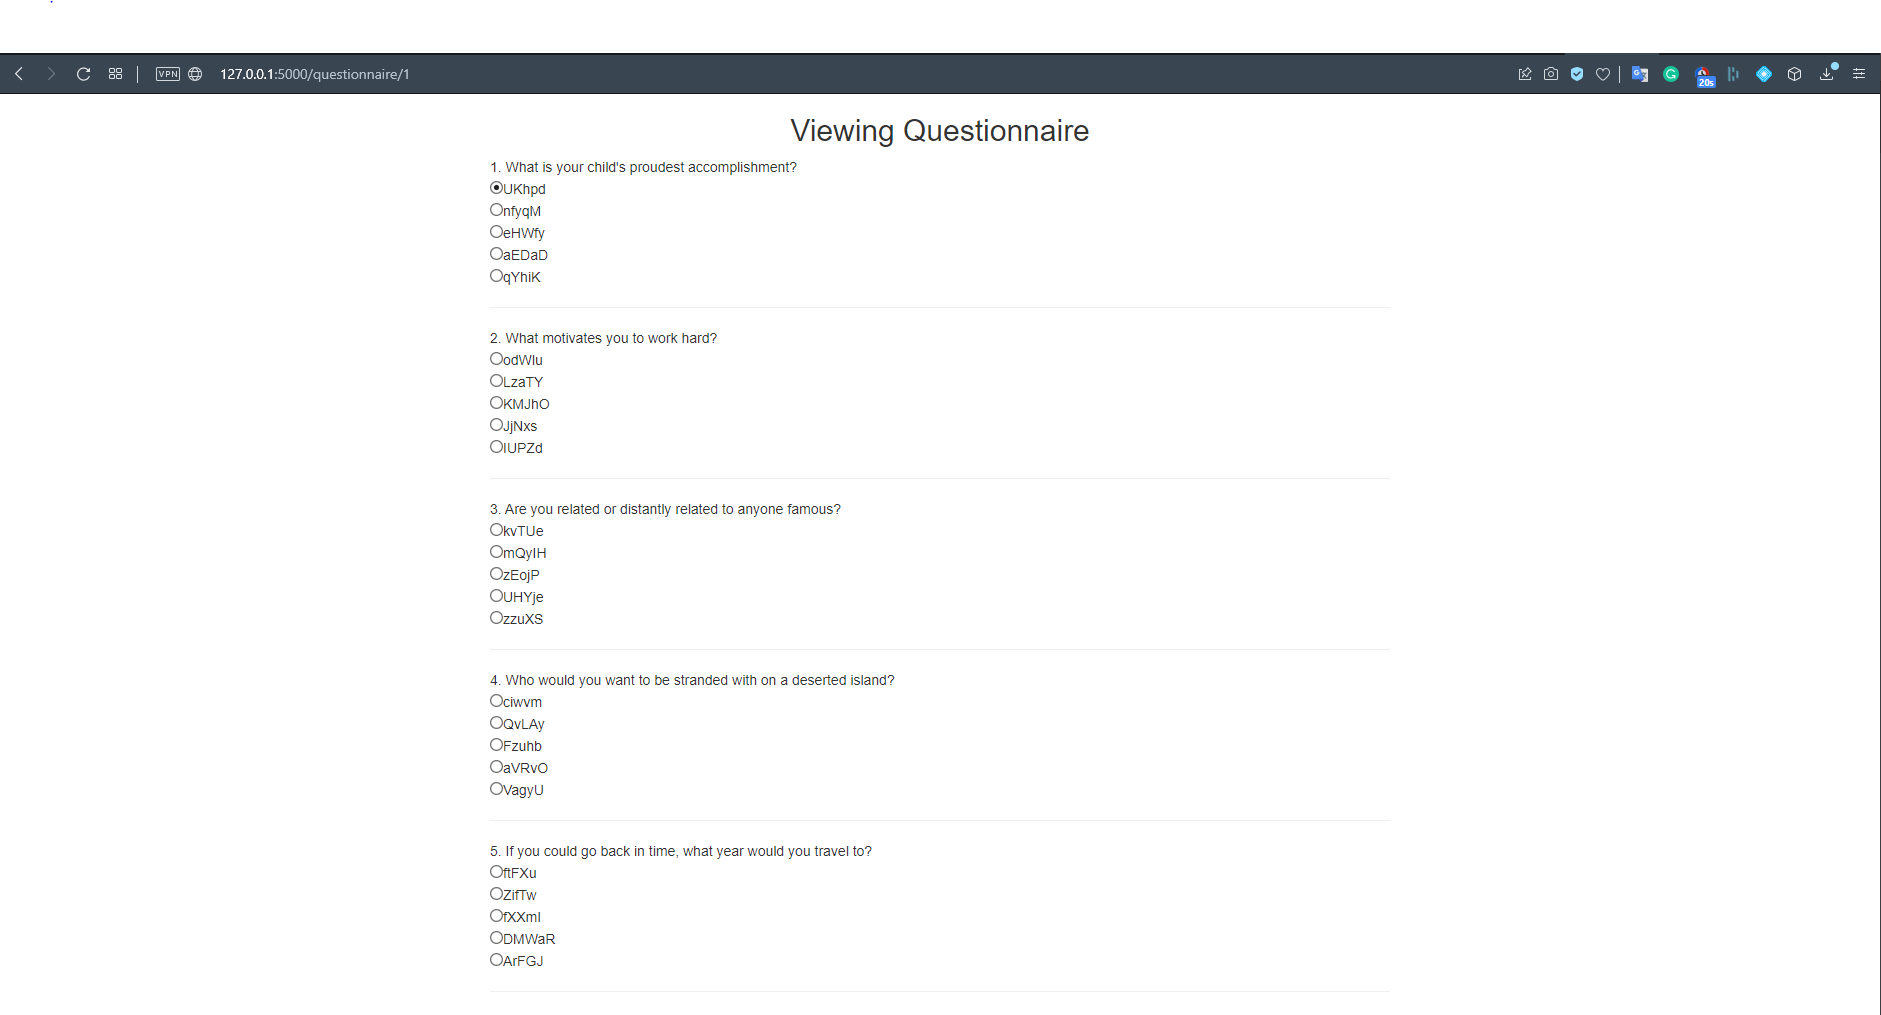
\includegraphics[width=\textwidth]{web_questionnaire.PNG}
        }
    \end{figure}

    %%%%%%%%%%%%%%%%%%%%%%%%%%%%%%%%%%%%%%%%%%%%%%%%%%%%%%%%%%%%%%%%%%%%%%%%%%
    %%%%%%%%%%%%%%%%%%%%%%%%%%%%%%%%%%%%%%%%%%%%%%%%%%%%%%%%%%%%%%%%%%%%%%%%%%
    %%%%%%%%%%%%%%%%%%%%%%%%%%%%%%%%%%%%%%%%%%%%%%%%%%%%%%%%%%%%%%%%%%%%%%%%%%
    \section{Console App}
    \FloatBarrier
    \begin{figure}[H] 
        \centerline{
        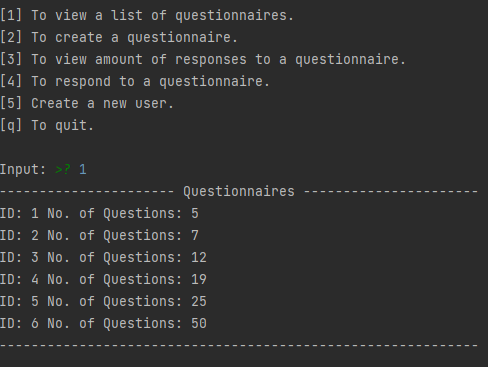
\includegraphics[width=\textwidth]{console_list_of_questionnaires.PNG}
        }
    \end{figure}
    \FloatBarrier
    \begin{figure}[H] 
        \centerline{
        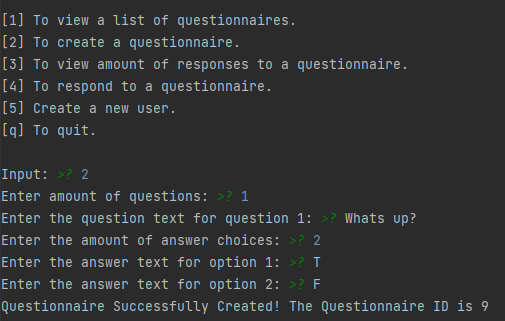
\includegraphics[width=\textwidth]{console_create_questionnaire.PNG}
        }
    \end{figure}
    \FloatBarrier
    \begin{figure}[H] 
        \centerline{
        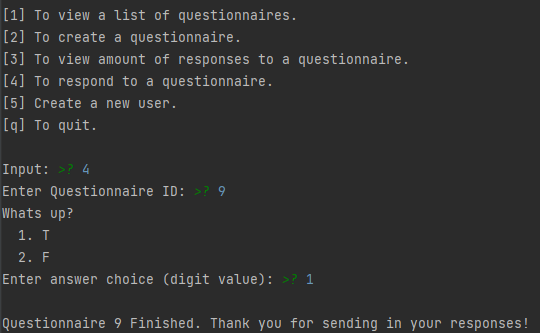
\includegraphics[width=\textwidth]{console_response.PNG}
        }
    \end{figure}
    \FloatBarrier
    \begin{figure}[H] 
        \centerline{
        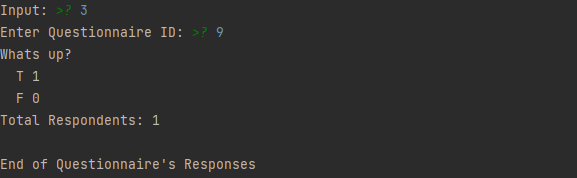
\includegraphics[width=\textwidth]{console_stats.PNG}
        }
    \end{figure}
    \FloatBarrier
    \begin{figure}[H] 
        \centerline{
        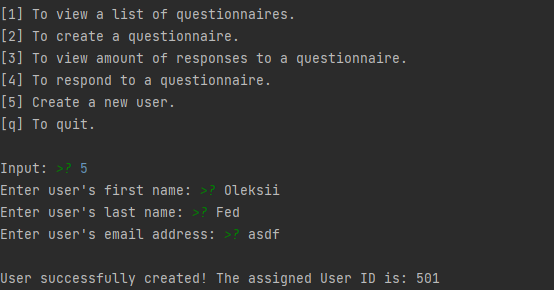
\includegraphics[width=\textwidth]{console_create_user.PNG}
        }
    \end{figure}

    %%%%%%%%%%%%%%%%%%%%%%%%%%%%%%%%%%%%%%%%%%%%%%%%%%%%%%%%%%%%%%%%%%%%%%%%%%
    %%%%%%%%%%%%%%%%%%%%%%%%%%%%%%%%%%%%%%%%%%%%%%%%%%%%%%%%%%%%%%%%%%%%%%%%%%
    %%%%%%%%%%%%%%%%%%%%%%%%%%%%%%%%%%%%%%%%%%%%%%%%%%%%%%%%%%%%%%%%%%%%%%%%%%
    \section{Contributions of Each Team Member}
    Oleksii:
    \begin{outline}
        \1 Database structure
        \1 Initial ER diagram
        \1 ER to SQL Tables
        \1 Helped with Functional Dependencies
        \1 Wrote script to generate sample data
        \1 Set up and worked on the Python Flask
        \1 Helped with writing samle queries
        \1 Helped with final report
    \end{outline}
    David:
    \begin{outline}
        \1 Sample queries, including SQL, RA, and TRC queries
        \1 Background section of report
        \1 Data description
        \1 Final report
    \end{outline}
    Matthew:
    \begin{outline}
        \1 Helped with initial design of database structure for initial report
        \1 Created sample queries with SQL code and did RA, TRC for one
        \1 Creation of console app in Python
        \1 Created and tweaked sample queries for usage in console app
        \1 Worked on the Python Flask
        \1 Helped with final report
    \end{outline}
    Preeti:
    \begin{outline}
        \1 Helped with initial Report
        \1 Helped with initial ER diagram
        \1 Wrote sections of the script for the presentation
        \1 Helped with presentation creation
    \end{outline}
    %%%%%%%%%%%%%%%%%%%%%%%%%%%%%%%%%%%%%%%%%%%%%%%%%%%%%%%%%%%%%%%%%%%%%%%%%%
    %%%%%%%%%%%%%%%%%%%%%%%%%%%%%%%%%%%%%%%%%%%%%%%%%%%%%%%%%%%%%%%%%%%%%%%%%%
    %%%%%%%%%%%%%%%%%%%%%%%%%%%%%%%%%%%%%%%%%%%%%%%%%%%%%%%%%%%%%%%%%%%%%%%%%%
    \section{What We Learned}
    During the course of this project, we learned about how to design our own database system and how to connect the many parts of our project and application together. The lectures taught us how to analyze and describe databases, schemas, and ER diagrams that other people have already made, but the project required us to create our own project and then design a database from scratch for it. The course helped a lot with the theory behind designing a database such as through the rules for ER diagrams and normal forms for schemas, but working on the project gave us the practical experience of actually creating our own database system. We also learned how to use MySQL for our project. Additionally, we learned about how to create web apps using Flask and how to connect MySQL to Python through SQLAlchemy.


\end{document}